\label{sec:4.1}

%%%%%%%%%%%%%%%%%%%%%%%%%%%%%%%%%%%%%%%%%%%%%%%%%%%%%%%
%(GAO) Discuss noise performance
%%%%%%%%%%%%%%%%%%%%%%%%%%%%%%%%%%%%%%%%%%%%%%%%%%%%%%%

\subsubsection{ColdADC Only}
The noise distribution for 16-channels from one ColdADC chip with the input floating are shown in Figure~\ref{fig:qc_noisewarm} (RT) and Figure~\ref{fig:qc_noisecold} (LN$_2$). The results are given in full 16-bit ADC output. The average noise is 6.7 LSB (302 $\mu$V-rms) at warm and 4.2 LSB (189 $\mu$V-rms) in LN$_2$, in 16-bit. The measurement is done with ColdADC configured after calibration, VDDA2P5/VDDD2P5=2.5 V, VDDD1P2=2.0 V, VDDIO=2.25 V, SDC bypassed. Separate study has shown that SDC noise is negligible. 
\begin{figure}[h!]
\centering
  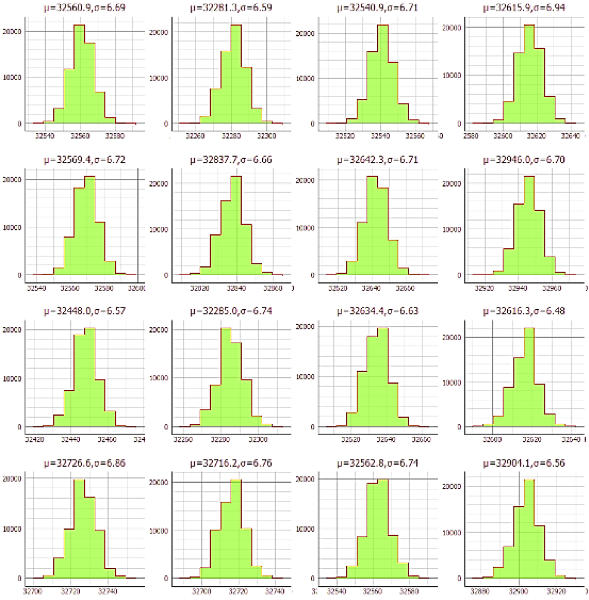
\includegraphics[width=0.8\linewidth]{figures/qc_noisewarm.png}
  \caption{Noise distribution (16-bit) of 16 input channels at room temperature.}
  \label{fig:qc_noisewarm}
\end{figure}
\begin{figure}[h!]
\centering
  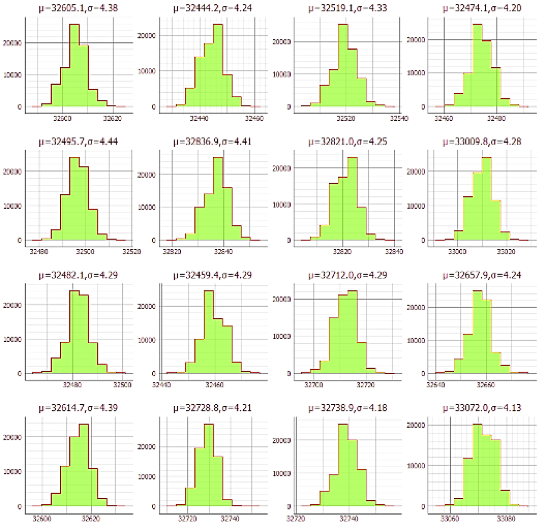
\includegraphics[width=0.8\linewidth]{figures/qc_noisecold.png}
  \caption{Noise distribution (16-bit) of 16 input channels at LN$_2$ temperature.}
  \label{fig:qc_noisecold}
\end{figure}



\subsubsection{LArASIC + ColdADC}
